\documentclass[conference]{IEEEtran}
\usepackage[T1]{fontenc}
\usepackage[utf8]{inputenc}
\usepackage{amsmath,amssymb,graphicx,booktabs,cite}
\usepackage[hidelinks,breaklinks]{hyperref}
\usepackage{url}
\newcommand{\E}{\mathbb{E}}
\newcommand{\Prob}{\mathbb{P}}
\newcommand{\Hist}{\mathcal{H}}
\newcommand{\ind}{\mathbf{1}}
\newcommand{\pr}[1]{\textsf{#1}}
\renewcommand{\thesection}{S\arabic{section}}
\renewcommand{\thetable}{S\arabic{table}}
\renewcommand{\thefigure}{S\arabic{figure}}
\renewcommand{\theequation}{S\arabic{equation}}
\title{Supplementary Material for ``Task-Aware Reuse of Cellular Molecular Receivers: Response Prediction and Feedback-Driven Waiting''}
\author{\IEEEauthorblockN{Ruifeng Zheng}\IEEEauthorblockA{Deutsche Telekom Chair of Communication Networks\\TU Dresden, Germany}}
\begin{document}
\maketitle

This supplement collects the implementation details, secondary analyses and sensitivity results behind the paper. Numbers without the prefix S refer to the paper. Every analysis was frozen in its own protocol before its only run (\texttt{simulation/configs}) and is checked by a verification script; as in the paper, every number printed with four or more decimals is checked against the frozen reference, and the reported values are recomputed by \texttt{python scripts/reproduce.py --mode verify}.

\section{Predictors, Data and Scores}
\label{sec:s-data}
\begin{table}[t]
\caption{Nested predictors and their features.}
\label{tab:s-features}
\centering\footnotesize\setlength{\tabcolsep}{3pt}
\begin{tabular}{lccccc}
\toprule
Predictor & $u_t,y_t$, slope & $\bar y_\ell$ & lags & $\hat\delta_{t,h}$ & $v_\ell$, $\int u$\\
\midrule
\pr{Persist} ($\hat y_{t+h}=y_t$) & & & & & \\
\pr{Current} & \checkmark & & & & \\
\pr{Filter} & \checkmark & \checkmark & & & \\
\pr{Lag} & \checkmark & & \checkmark & & \\
\pr{Filter+B3} & \checkmark & \checkmark & & \checkmark & \\
\pr{Lag+B3} & \checkmark & & \checkmark & \checkmark & \\
\pr{F+B3+Input} & \checkmark & \checkmark & & \checkmark & \checkmark \\
\bottomrule
\end{tabular}
\end{table}

Predictors for horizons $h\in\{2,10,20,30\}$~min start after a fixed 10-min warmup; future reporters are targets only. Table~\ref{tab:s-features} lists the feature sets (slope: last reporter increment per minute; $\int u$: cumulative command; repository code keys P, C, O, A, M, A+M and H, in table order); every learned predictor also receives the known future command and is fitted by ridge regression with equal weight per condition. Lags are the reporter and command values of the previous 5--30 frames. The causal reporter and input filters with scales $\ell\in\{2,10,60\}$~min are those of Eq.~(4) of the paper, and the B3 increment of Eq.~(5) of the paper weights the authors' 1,000 posterior samples by the cell's past reporter, a fixed-parameter particle approximation of the B3 belief that uses the same information as the learned predictors. Since $\hat\delta_{t,h}$ already uses the command history, \pr{F+B3+Input} tests only the extra value of explicit input features. Penalty, $\sigma$ and lag length are chosen on validation data; normalization, lag filling and fitting details are in the repository.

All numerical files come from the paper-linked repository at a pinned commit \cite{lfnsrepo,mendeley2020}; commands follow the authors' model XML, and per-cell normalization uses only frames before stimulation onset. Table~\ref{tab:s-inventory} lists the 22 conditions with their roles and cell counts (1,565 cells in total, 2-min frames). Roles were frozen before any newly used response file was downloaded: Test A is a new protocol, Test B's timing was inferred from the authors' simulations, and Test C uses new concentrations recorded in the session of the inspected mixed blocks (role ``Viewed''). Because the authors fitted B3 to the sustained and 3/20 means and compared architectures on the single 5-min and mixed blocks at 2.5 and 250~ng/ml (``fit'' and ``arch.'' in the last column of Table~\ref{tab:s-inventory}), B3 is a calibrated reference, not a model blind to those protocols; it is executed from the authors' files without refitting (posterior-predictive mean within $8.5\times10^{-6}$ of their exports). In the corrected leave-one-protocol-out (LOPO) each of six protocol groups is held out with predictor tuning restricted to the remaining protocols. Forecast rows are assigned to the phases stimulation, next command (a pulse starts in $(t,t+h]$), early washout ($\le30$~min after a pulse) and late. The score is the square root of the equally weighted condition MSE,
\begin{equation}
 \mathrm{RMSE}(h)=\Big[\tfrac{1}{|\mathcal{K}|}\textstyle\sum_{k\in\mathcal{K}}\tfrac{1}{N_{k,h}}\sum_{i\in k}(\hat y_{i+h}-y_{i+h})^2\Big]^{1/2},
 \label{eq:s-score}
\end{equation}
over the conditions $\mathcal{K}$ of a role. Because every error contains the reporter noise, we also report a noise-adjusted skill, $1-\overline{(\mathrm{MSE}-\hat\sigma_\nu^2)}/\overline{(\mathrm{MSE}_{\rm Persist}-\hat\sigma_\nu^2)}$, with $\hat\sigma_\nu$ a robust second-difference estimate of white reporter noise per condition (0.006--0.009), and 95\% intervals from resampling cells within conditions. Cells share a session and no day identifiers exist, so intervals describe cell sampling, not independent experiments. Every analysis was frozen in its own protocol before running, but all are post hoc with respect to inspected data.

\begin{table}[t]
\caption{Protocols, roles and cells (``fit'' and ``arch.'': B3 fitting and architecture comparison by the original authors).}
\label{tab:s-inventory}
\centering\footnotesize\setlength{\tabcolsep}{3pt}
\begin{tabular}{lllrl}
\toprule
Protocol & Role & ng/ml & Cells & B3 use \\
\midrule
Sustained & Train & 0.25, 2.5, 25, 250 & 248 & fit 2.5, 250 \\
3/20 pulses & Train & 2.5, 25, 250 & 207 & fit 2.5, 250 \\
Single 5 min & Val. & 0.25, 2.5, 25, 250 & 370 & arch. 2.5, 250 \\
Single 10 min & Test A & 0.25, 2.5, 25, 250 & 248 & -- \\
Single 60 min & Test B & 2.5, 25, 250 & 167 & -- \\
Mixed & Test C & 0.25, 25 & 171 & -- \\
Mixed & Viewed & 2.5, 250 & 154 & arch. 2.5, 250 \\
\bottomrule
\end{tabular}

\end{table}

\section{Which Information Predicts the Response}
\label{sec:s-forecast}
\begin{table}[t]
\caption{10-min RMSE in the corrected leave-one-protocol-out analysis.}
\label{tab:s-lopo}
\centering\footnotesize\setlength{\tabcolsep}{2.5pt}
\begin{tabular}{lcccl}
\toprule
Held-out protocol & O & M & H & B3 prior use \\
\midrule
Sustained & 0.02102 & 0.01969 & \textbf{0.01941} & fit 2.5, 250 \\
3/20 pulses & 0.03680 & 0.02886 & \textbf{0.02830} & fit 2.5, 250 \\
Single 5 min & 0.02243 & 0.02153 & \textbf{0.02139} & arch. 2.5, 250 \\
Single 10 min & \textbf{0.02084} & 0.02106 & 0.02104 & none \\
Single 60 min & 0.02701 & 0.02410 & \textbf{0.02369} & none \\
Mixed, 0.25/25 & 0.02709 & 0.02623 & \textbf{0.02610} & other conc. arch. \\
\bottomrule
\end{tabular}

\end{table}

\begin{figure}[t]
\centering
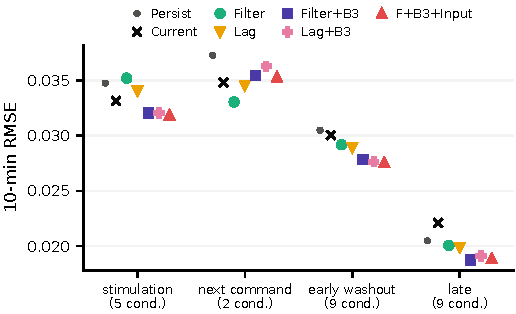
\includegraphics[width=\columnwidth]{figures/prediction_phases.pdf}
\caption{(a) Condition-equal 10-min RMSE on Tests A--C by forecast phase (axis not starting at zero). (b) Noise-adjusted skill on Test A by forecast horizon; band: 95\% cell-bootstrap interval of \pr{Filter+B3}.}
\label{fig:s-phases}
\end{figure}

Table~I of the paper reports the RMSE of Eq.~\eqref{eq:s-score} at 10~min for the validation (Val.) and test roles (A--C) of Table~\ref{tab:s-inventory} (last column: 2~min on Test A); bold marks the best predictor per column, and the bottom rows count the conditions in which the first predictor of each pair has the lower MSE. The most robust result is that \pr{Filter+B3} beat persistence on all four roles, by 6.7--7.6\%, and that the B3 increment carried this gain: it lowered the error of \pr{Filter} on every role (4.5--9.8\%), whereas filtering helped only on the validation protocol and Test A (4.0\% and 9.1\%; none on Tests B and C at 10~min, although at 2, 20 and 30~min it helped on all four), and \pr{Filter} beat persistence only on Tests A and C (by 2.9\% and 1.7\%) because \pr{Current} was itself worse than \pr{Persist} on three roles. On Test A at 10~min, reporter filtering reduced the error by 9.1\% relative to \pr{Current}, the B3 increment by 4.5\% relative to \pr{Filter}, and input history by 1.0\% relative to \pr{Filter+B3}, giving 0.02098, 8.2\% below \pr{Persist}; these reductions use different baselines and are not additive. On the MSE scale the three Test A reductions are 17.3\%, 8.9\% and 2.0\%; subtracting the white-noise floor, under a tenth of the \pr{Persist} MSE at 10~min, raises them only to 18.8\%, 9.8\% and 2.2\%. \pr{Filter+B3} explains 15.5\% of the noise-free \pr{Persist} error (Fig.~\ref{fig:s-phases}(b) gives this noise-adjusted skill by horizon, with a 95\% cell-bootstrap interval for \pr{Filter+B3}), and the cell-bootstrap intervals of the three RMSE reductions were 7.4--10.9\%, 3.0--6.1\% and 0.6--1.4\%. The input-history gain was small and not consistent across conditions (two of four on Test A; 0.4\% and 0.1\% on B and C). The lagged baseline \pr{Lag} was 2.3\% worse than \pr{Filter} on Test A, but adding the B3 increment to it still reduced the error by 6.9\% (four of four concentrations), so on Test A the mechanistic gain holds for both the filter and the lag representation of the history. In the corrected LOPO (Table~\ref{tab:s-lopo}, where F+B3 and F+B3+In abbreviate \pr{Filter+B3} and \pr{F+B3+Input}; bold: best per held-out protocol; last column: B3's prior use of that protocol, with $^\circ$ marking use at other concentrations), \pr{F+B3+Input} beat \pr{Filter+B3} in all six folds (by 0.1--2.0\%) and \pr{Lag+B3} beat \pr{Lag} in all six, but with the 10-min pulse held out, one of the two protocols unseen by B3, \pr{Filter+B3} was 1.1\% worse than \pr{Filter}. At longer horizons the mechanistic increment mattered more (Fig.~\ref{fig:s-phases}(b)): on Test A its skill rose to 21\% at 20 and 30~min against 9--13\% for \pr{Filter}, and it anticipated the half-decay crossing of the reporter more often (balanced accuracy 57--58\% versus 52--53\%; 65--67\% versus 54--57\% on Test B), although no predictor did so reliably. Explicit input history became harmful on Tests A and B: \pr{F+B3+Input} fell to $-1.7\%$ skill at 20~min on Test A and to $-50\%$ and $-53\%$ on Test B at 20 and 30~min, although on Test C it lowered the 20- and 30-min error by 3.6\% and 3.0\%.

\section{The Next-Command Window}
\label{sec:s-nextcmd}
By phase (Fig.~\ref{fig:s-phases}), the B3 increment reduced the error of \pr{Filter} during stimulation (8.9\%), early washout (4.6\%) and the late phase (6.6\%), but raised it in the next-command window from 0.03306 to 0.03544; at 2, 20 and 30~min it lowered the next-command error (by 2.9\%, 4.0\% and 6.9\%), so the failure is specific to the 10-min horizon. That window holds two mixed conditions with ten forecast origins each, five before the 30-min pulse (20~min after the initial 3-min pulse) and five before the 5-min pulse that follows it after 60~min: the increment helped at 0.25~ng/ml (0.03652 to 0.03485) and hurt at 25~ng/ml (0.02920 to 0.03603). Two phase-gated variants fitted on the training protocols did not repair this: a switch to \pr{Filter} in next-command rows was rejected by the training data, where the increment helped (in-sample MSE $6.3\times10^{-4}$ versus $8.4\times10^{-4}$), and phase-specific weights (\pr{F+B3 (phase)} in Fig.~\ref{fig:s-phases}(b)) raised the next-command error to 0.03571 (held-out mixed fold: 0.03630, versus 0.03537 for \pr{Filter+B3} and 0.03302 for \pr{Filter}). The training protocols contain no probe after a long command, so their next-command windows cannot teach the correction. A frozen descriptive split of the window by the following pulse did not locate the increase. At 25~ng/ml the five origins before the 5-min pulse, 50--58~min after the 30-min pulse, carried 69\% of it, below the pre-specified 75\%; there the increment raised the error by 35\% (0.02737 to 0.03694; worse in 82 of 84 cells): it predicted a rise (mean $+0.013$) where the reporter fell ($-0.009$), so its forecasts were too high (mean error $+0.021$ versus $+0.015$ for \pr{Filter}), consistent with B3 overestimating recovery after the long command (Sec.~\ref{sec:s-natural}). Before the 30-min pulse it raised the error by 13.5\% (0.03092 to 0.03510; mean error $-0.003$, 95\% interval $-0.008$ to $+0.001$). The groups also differ in the following pulse, the time since the last pulse and the reporter history, and they are the probe cells of Sec.~\ref{sec:s-natural}, so the split is not independent evidence.

\section{Waiting under a Per-History Reliability Requirement}
\label{sec:s-waiting}
This section, Sec.~\ref{sec:s-delay} and Sec.~\ref{sec:s-mismatch} document the earlier evaluation, which split the 1,000 posterior rows into halves, left each receiver out of its own references by index and calibrated to empirical targets; the frontiers, the condition map and the mismatch study use it. Table~II of the paper comes from the strict evaluation of Sec.~\ref{sec:s-strict}.

\begin{figure*}[t]
\centering
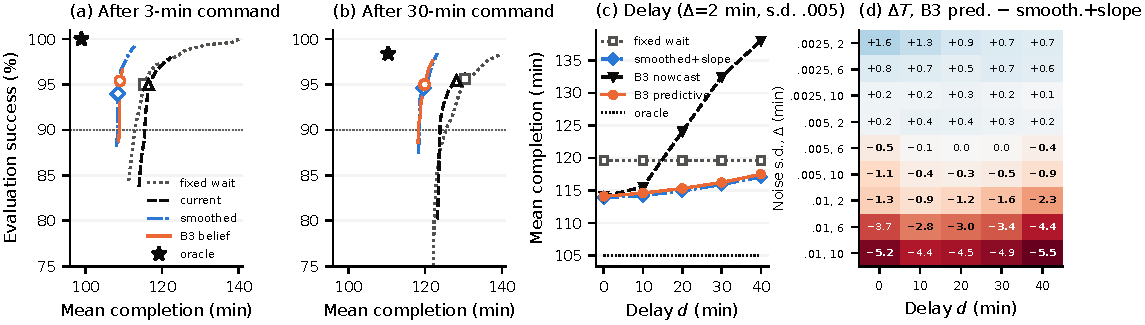
\includegraphics[width=\textwidth]{figures/waiting_frontier.pdf}
\caption{Waiting on the authors' B3 model (25~ng/ml; task: probe rise $\geq$ 50\% of the naive rise within 20~min). (a,b) Reliability--latency frontiers on evaluation samples (primary split, noise s.d.\ 0.005; thresholds or waits swept, descriptive), with the operating points calibrated to 0.94 (open markers). (c) Median completion over 20 splits versus feedback delay $d$ (calibration target 0.94 per history). (d) Condition map: median over splits of the paired completion difference, B3-predictive minus smoothed+slope (min; negative: the model is faster) over delay, noise s.d.\ and sampling interval $\Delta$; bold: model faster in $\geq$16 of 20 splits at no more than 0.5 points lower success at targets 0.94 and 0.90; n.c.: the B3 rule never reached the target after the 3-min command. One simulated model structure, not measured cells.}
\label{fig:s-waiting}
\end{figure*}

Rule details. Each rule probes at the first decision time at which its estimate reaches a threshold (Eq.~(6) of the paper), a stopping time on the observations, as in sequential tests \cite{wald1945}. Three estimators of $R_t$ are compared on B3: \emph{current} uses only $y_t$, through a Gaussian kernel over the (reporter, success) states of reference receivers; \emph{smoothed} applies the same kernel to a causal exponential smoothing of the observations (scale 2--16~min); the \emph{B3 belief} weights reference receivers under the known command history by all observations, as in Eq.~(5) of the paper, with likelihood s.d.\ equal to the noise s.d.\ floored at 0.001. The comparator is one fixed wait per previous command, a history-conditioned guard interval. References are one half of the posterior samples (calibration; each receiver left out of its own references); the other half (evaluation) never enters references, thresholds or waits. Every rule, fixed or adaptive, chooses its parameters per previous command (a wait, a threshold, or for smoothing a scale and a threshold) to minimize that history's calibration completion subject to its calibration success $\geq$ a target, i.e.\ Eq.~(3) of the paper on calibration samples. Twenty splits redraw the halves and the observation noise. With delay $d$, the \emph{B3-predictive} rule averages the references' success at $t+d$ under the same weights, $\widehat R_{t+d\mid t}=\sum_s w_s(t)S_s(t+d)$; the \emph{B3 nowcast} ignores the delay. The comparator without a command-history model, \emph{smoothing plus slope}, also extrapolates: a kernel over the smoothed level and its last increment, $(\bar y_t,\bar y_t-\bar y_{t-\Delta})$, with the covariance of smoothed white noise, maps the current trend to success at $t+d$. Observations arrive every $\Delta\in\{2,6,10\}$~min and decisions are made when they arrive.

Choice of the task threshold. We use $\kappa=0.5$, fixed before the waiting analyses after $\kappa=0.8$ proved infeasible; a later scan over $\{0.30,0.35,\ldots,0.70\}$ shows that it is also the largest value at which an oracle, which probes at the first decision time at which the probe would succeed, still succeeds for $>99\%$ of simulated receivers within 120~min, pooled over both histories (99.25\%, 98.5\% after the 30-min command; 95.1\% at 0.55, 82.0\% at 0.60).

Readiness and waiting were simulated on B3 with 25~ng/ml commands and observations every 2~min. Readiness depended almost only on the current reporter, waits of 6--48~min never succeeded, and no state met the criterion without the probe. In Fig.~\ref{fig:s-waiting}(a,b) the smoothed and B3-belief frontiers lie between the fixed waits and the oracle and nearly coincide, whereas the current-observation frontier is no better than the fixed waits after the 3-min command and better only at 90\% success or above after the 30-min command. Calibrated to 0.90, every rule, fixed waits included, met 0.9 for both histories in only 7--11 of 20 splits, so a calibration target equal to the requirement leaves no margin. At 0.94 all rules met it in every split at noise 0.005, which is why the earlier version tabulated this target (Table~\ref{tab:s-old}), a choice made after the splits were evaluated; the paper now uses the certified calibration of Sec.~\ref{sec:s-strict}. Table~\ref{tab:s-old} gives, for each rule (``Current obs.'': the current estimator), the evaluation success $S_m$ (\%) and mean completion $T_m$ (min) after the $m$-min command on the primary split at the reference noise s.d.\ 0.005 (lower block: 0.01 with the same fixed waits) and, as medians over the 20 splits, the difference $\Delta T=T_{\rm rule}-T_{\rm fix}$ in mean completion $T$ over both histories (negative: earlier), the closed share $G=(T_{\rm fix}-T_{\rm rule})/(T_{\rm fix}-T_{\rm oracle})$ of the gap to the oracle, and the number of splits (Met) with $S_3,S_{30}\geq90\%$. Feedback finished 7.2~min (B3 belief) and 7.7~min (smoothed) earlier than per-history fixed waits (94 and 110~min on the primary split), faster in all 20 splits, and closed 42\% and 45\% of the gap to the oracle. At the other pre-specified targets, 0.90 and 0.92, where the requirement was met in 7--11 and 16--19 of 20 splits, feedback closed 38--42\% of the gap (saving 5.5--6.6~min), again faster in all 20 splits. The current-reporter rule closed none of it. Under a pooled requirement (success averaged over both histories), the B3 belief and smoothing closed 33\% and 38\% of the gap between pooled history-conditioned waits and the oracle (4.8 and 5.5~min; primary split). At noise s.d.\ 0.01 the B3 belief beat smoothing in all splits at every target (split medians 1.5--1.7~min; 30--35\% versus 21--26\% of the gap), whereas at 0.005 smoothing was 0.2--0.4~min faster. Larger failure penalties ($T_{\rm f}=160$--260~min, target 0.90) raised the B3 belief's gain over fixed waits from 5.5 to 5.9--8.7~min, with the smoothed and B3-belief rules still ahead of the fixed waits. Sensitivity analyses with pooled calibration (repository) agree: the gain persists at $\kappa=0.4$ and at a shared calibration margin, at $\kappa=0.6$ even the oracle fails for about 18\% of receivers, and under correlated noise the B3 belief needs a likelihood that models the correlation (median success over 20 splits 81\% with frozen thresholds and 92\% with an AR(1) likelihood, which met 0.9 in 13 of 20 splits), whereas the smoothed rule recovers by recalibration alone (19 of 20).

\section{Delay, Noise and Sampling}
\label{sec:s-delay}
With delay, readiness must be predicted. The condition map was first frozen and run with every rule calibrated to 0.90 per history, at which the requirement was met in only part of the splits, and then re-run at 0.92 and 0.94 under a second frozen protocol; we report 0.94, as in the earlier evaluation (Table~\ref{tab:s-old}), a target chosen after the first evaluation. The B3 nowcast became slower than the fixed waits from $d=20$~min on (124--138 versus 122~min), whereas both predictive rules lost only about 4~min between $d=0$ and 40~min (Fig.~\ref{fig:s-waiting}(c)), so the value of feedback over fixed waits shrank from 7.2--7.9 to 3.1--3.8~min. The condition map (Fig.~\ref{fig:s-waiting}(d)) answers when the model is needed. At noise s.d.\ 0.01 the B3-predictive rule was faster than smoothing plus slope in every split of every cell, by 0.9--5.4~min, and the smoothing-plus-slope rule became slower than the fixed waits with 10-min sampling, from $d=20$~min with 6-min sampling and at $d=40$~min with 2-min sampling (by 0.4--4.7~min), while the B3-predictive rule still beat them (by 1.0--2.8~min). At the reference noise the model helped with 10-min sampling at every delay (0.4--1.1~min) and with 6-min sampling only without delay (0.5~min); with 2-min sampling at the reference noise and with 6- or 10-min sampling at noise 0.0025 the smoothed trend was 0.2--0.7~min faster. At noise 0.0025 with 2-min sampling the B3-predictive rule never reached the target after the 3-min command on calibration (median evaluation success 87.6--90.2\%), consistent with weight collapse at low noise, so these five cells are not classified; elsewhere the fixed waits met the requirement in all 20 splits and the B3-predictive and smoothing-plus-slope rules in 19 or 20. The model was faster in at least 16 of 20 splits in 21 of the 45 cells and also no more than 0.5 points below the smoothing-plus-slope rule's median success in 18 of them; the other three, all at noise 0.01, had 0.6--1.6 points lower median success. Seventeen of the 18 were also selected at 0.90 and are bold in Fig.~\ref{fig:s-waiting}(d); two cells (0.005/6/40 and 0.01/10/30) change class between 0.90 and 0.94. At 0.92, where fixed waits met the requirement in 17 and smoothing plus slope in 13--19 of 20 splits, only 10 of the 17 kept this class (and 0.01/6/0 joined it); in the other seven the B3 rule was still faster in 19 or 20 splits but met the requirement in only 13--15 or had more than 0.5 points lower median success, so the gain at the reference noise depends on the calibration margin. The success condition, on pooled median success, limits but does not rule out trading reliability for speed after one history.

\section{Natural Probes, Posterior Predictive Check and Weight Collapse}
\label{sec:s-natural}
Two recorded protocols contain later pulses that act as probes at fixed waits (25~ng/ml): in the 3/20 protocol each 3-min pulse comes 20~min after the previous one, with the cell's own first-pulse rise as naive reference (58 cells); in the mixed protocol (84 cells) a 5-min pulse comes 60~min after a 30-min pulse, scored against single 5-min pulse cells (92 cells). Both probes were early by B3's standard: B3 predicted no success for any sample, and every estimator called no cell ready. The measured cells agreed: 19\% met the criterion at the first 3/20 probe and 3--9\% at later ones, and none at the mixed probe, so the rules made no false ready call but missed the 19\%. The rises differed, however: at the mixed probe measured cells reached a median 4\% of the naive rise where B3 predicts 31\%, consistent with B3 overestimating recovery after a long command. These cells also supply the 25~ng/ml next-command window, in which the increment over-predicted the reporter before this probe (Sec.~\ref{sec:s-nextcmd}), so the probe and that forecast error are not independent evidence. After a short pulse B3 erred the other way: at the first 3/20 probe it underestimated the rise (8\% versus 16\% of the naive rise). A posterior predictive check across doses (Fig.~3(a) of the paper), frozen after an exploratory look at the same quantities, locates the error. Sixty minutes after a 30-min pulse the measured probe rise was 4\% and 8\% of the naive rise at 25 and 250~ng/ml (95\% intervals 2--8\% and 4--14\%), indistinguishable from no response and below all 1,000 posterior samples (5--95\% ranges 23--39\% and 27--40\%), whereas at 2.5~ng/ml it lay within B3's range (36\% versus 35--48\%). After a 3-min pulse the measured recovery lay within or at the edge of B3's range at the doses B3 was fitted to (87\% versus 73--90\% at 2.5~ng/ml, 4\% versus 5--9\% at 250~ng/ml) and above it only at 25~ng/ml, with overlapping intervals. B3 thus errs where its fit gave it no data, recovery after a long, strong command, which is the regime that matters for reuse, and no reweighting of its samples can repair this. The B3 weights collapsed on measured cells (effective sample size 1.0--1.4), as on the cells B3 was fitted to (1.1--2.3): the posterior's reporter spread (0.001--0.004) lay below the noise floor, whereas the best sample left residuals 3.2--5.3 times the noise floor that were correlated in time (lag-1 autocorrelation 0.22--0.77). A per-cell gain and offset removed the collapse only for the 3/20 cells at 2.5~ng/ml (effective sample size 146); elsewhere residuals stayed 2.5--3.6 times the noise floor, so the pre-specified attribution to deviations that the posterior does not represent failed for one of four fitted conditions. A real-data filter therefore needs process noise or cell heterogeneity, and the measured noise floor (0.007--0.008) lies between the map's reference and high noise, where with 2-min sampling the map turns from the smoothed trend to the model, which would help only if it were right about recovery (the map was not re-run under the recovery errors of Sec.~\ref{sec:s-mismatch}).

\section{When the Model Misjudges Recovery}
\label{sec:s-mismatch}
Every waiting rule above, fixed waits included, is calibrated on B3 outcomes, so none is model-free, and Sec.~\ref{sec:s-natural} suggests that B3 recovers too fast after a long command. A frozen simulation therefore delayed the outcomes after the 30-min command by a lag $L$ that the reporter does not show (target 0.94, noise 0.005, 20 splits). Fixed waits and the current-reporter rule kept the per-history requirement up to $L=2$~min (in 20 and 17 of 20 splits; Fig.~3(b) of the paper), whereas the smoothed and B3-belief rules met it in only 10 and 15 of 20 splits at 2~min, and at $L=4$~min their success after the 30-min command fell from 95\% to 84--85\%, against 94\% to 89\% for the fixed waits, which then met the requirement in 8 of 20 splits. The smoothed and B3-belief rules save time by probing soon after readiness and so leave less slack, the time from readiness to the probe, for a recovery error that the reporter hides. Read as a pure time shift, the measured mixed probe corresponds to a B3-equivalent lag of about 35.5~min: B3's posterior-median rise reaches the measured 4\% at a wait of 24.5 instead of 60~min. One probe cannot separate a delay from a loss of amplitude, a slowing or a mixture of responders, and the 4\% rise lies within the interquartile range of rises expected from noise alone, so this is an equivalent value, not a bound (Sec.~\ref{sec:s-scope} fits the same point as an amplitude loss or a slowing). At that lag even the oracle succeeds for at most 31\% of receivers after the 30-min command within 120~min, and every rule failed. These are the cells of Sec.~\ref{sec:s-natural} and of the next-command window, not independent evidence. Recalibrating only the thresholds on true outcomes restored the requirement up to 6~min for the smoothed and current rules and 4~min for the B3 belief, and recalibrated fixed waits kept it up to 14~min; adding a post-trigger delay $\delta$ (the probe acts at $\min(\tau+\delta,120)$ with $\tau$ from Eq.~(6) of the paper), calibrated together with the threshold, restored it for all three feedback rules in 18--20 of 20 splits up to $L=12$~min (recalibration was feasible in every split up to 10~min and in 12 at 12~min), with the smoothed and B3-belief rules 6.2--7.7~min faster than recalibrated fixed waits. This uses the complete outcome curves of the calibration receivers and a common lag, an ideal-information benchmark for calibration from measured probes, which Sec.~\ref{sec:s-budget} limits to one probe per receiver. When the lag also delays the reporter, the smoothed and current rules kept the requirement up to $L=8$~min (19--20 of 20 splits), the B3 belief up to 4~min and fixed waits not even at 4~min (8 of 20); at noise 0.01 the B3 belief lost more success than smoothing in 17 and 19 of 20 splits at 12 and 16~min (at 16~min the task was feasible in only 4 of 20 splits), while its effective sample size fell to 16 and 6.7. With the model correct, for the slowest quarter of receivers (readiness onset $\geq98$~min after the 30-min command) only the current rule met the requirement in any split (7 of 20), but the B3-belief and smoothed rules raised success after the 30-min command above that of the fixed waits (by 5.5 and 7.1 points, in 18 and 16 of 20 splits; for the slowest half by 2.2 and 0.4 points, in 13 and 10). Feedback thus absorbs recovery variation that the reporter shows, not a recovery error that it hides.

\section{Protocol Trace, Receivers and Task Definitions}
\label{sec:s-audit}
\begin{table}[t]
\caption{Commanded schedules used as model input (every dose has the same timing), in min from the origin of the truncated records; origin in raw minutes. Sources: P, recorded pulse file; X, B3 XML input; S, the authors' simulation summary.}
\label{tab:s-protocols}
\centering\footnotesize\setlength{\tabcolsep}{2.5pt}
\begin{tabular}{llll}
\toprule
Protocol & Pulses & Origin & Sources \\
\midrule
Sustained & $[0,\infty)$ & 43 & X, S \\
3/20 & 3~min every 23~min from 0 & 43 & X, S \\
Single 5-min & $[0,5)$ & 43 & X, S \\
Single 10-min & $[0,10)$ & 43 & X, S \\
Single 60-min & $[0,60)$ & 44 & S \\
Mixed & $[1,4)$, $[24,54)$, $[114,119)$ & 42 & P, X, S \\
\bottomrule
\end{tabular}
\end{table}

\begin{table}[t]
\caption{Measured natural probes versus the simulated task.}
\label{tab:s-task}
\centering\footnotesize\setlength{\tabcolsep}{2.2pt}
\begin{tabular}{p{1.25cm}p{2.1cm}p{2.1cm}p{2.1cm}}
\toprule
 & 3/20 probe & Mixed probe & Simulation \\
\midrule
Probe & 3~min, 20~min after a 3-min pulse & 5~min, 60~min after a 30-min pulse & 5~min after 3 or 30~min, wait 0--120~min \\
Naive rise & same cell, first pulse & median of other cells (single 5-min pulse) & same receiver, unstimulated \\
Response & noisy, 3-frame mean, 2-min frames & as 3/20 & noise-free, 1-min grid \\
Role & model check & model check & task of Eq.~(2) \\
\bottomrule
\end{tabular}
\end{table}

\emph{Stimulation protocols.} Every commanded schedule used here was traced to the authors' files (\texttt{audit\_protocols.py}; Table~\ref{tab:s-protocols}): the B3 XML inputs, the authors' simulation summary and, for the mixed protocol, the recorded pulse file. That file lists pulses at 43--46, 66--96 and 156--161~min of the raw recording. The authors' normalization script divides each cell by its median over raw 10--30~min and cuts the recording at its 22nd frame (42~min), which gives 1--4, 24--54 and 114--119~min, the schedule in the XML, the summary and our model input. Repeating this normalization on the raw records reproduces the truncated files at all four doses to the five significant digits in which they are stored, so the cut is the one applied to the data. Before the first pulse the reporter stayed at baseline: the median over cells of the largest deviation from 1 was 0.024--0.029, against a median rise of 0.13--0.15 within 20~min of the first pulse at 2.5--250~ng/ml, so no earlier, unrecorded stimulation is visible. Because the source paper describes the mixed protocol in two places that do not agree in detail, we rely on the recorded pulse file rather than either description. The other protocols have no pulse file; their XML and summary schedules agree with our input for all 23 condition schedules checked. Their truncated frames start 1~min after the onset (raw cut at 43~min), except the 60-min pulse, which has no XML input and whose frames start at its onset, an ambiguity of 1~min covered by the registered timing sensitivity. All schedules are commanded concentrations, not measured local concentrations.

\emph{Receivers and roles.} The author posterior file repeats 52 of its 1,000 rows (44 pairs and four triples; 948 distinct vectors). The earlier waiting evaluation split the rows into halves and left each receiver out of its own references by index, so 19--33 evaluation receivers per split had an identical twin among the references. Re-scoring that evaluation without them changed the median completion difference of the B3 belief against the fixed waits from $-7.19$ to $-7.11$~min and that of smoothing from $-7.71$ to $-7.69$~min (target 0.94), so the self-match was small; Table~\ref{tab:s-old} keeps the earlier table for reference. The evaluation of the paper uses the 948 distinct vectors with disjoint reference, calibration and test roles (Sec.~\ref{sec:s-strict}). A success probability there refers to a receiver drawn from these vectors with an independent draw of reporter noise: uncertainty about the population-mean parameters of one model structure, not cell-to-cell heterogeneity.

\emph{Infeasible calibration.} In the earlier evaluation every rule reached its calibration target in every split, so its fallback (the parameter with the highest calibration success) was never used. In the certified calibration, a history for which no parameter is admitted is probed at the 120-min horizon; such receivers stay in every success rate and completion time, and the number of fallbacks is reported with each result.

\emph{Task.} Table~\ref{tab:s-task} lists how the measured probes differ from the simulated task. They differ in probe length, naive reference and noise, and they are taken at fixed waits, so they check B3 but do not evaluate a waiting rule; only the simulations evaluate Eq.~(2) of the paper as defined. The recovery fraction $\kappa=0.5$ is a proxy for the next command's effect, not a biological function; Sec.~\ref{sec:s-scope} varies it with the window and the failure penalty.

\begin{table}[t]
\caption{Earlier evaluation (Table~II of the previous version): halves of the 1,000 posterior rows, leave-one-out references, target 0.94 chosen after evaluation. $\Delta T$, $G$ (gap to the oracle closed), Met: 20 splits.}
\label{tab:s-old}
\centering\footnotesize\setlength{\tabcolsep}{2.2pt}
\begin{tabular}{lccccccc}
\toprule
Rule & $S_3$ & $T_3$ & $S_{30}$ & $T_{30}$ & $\Delta T$ & $G$ (\%) & Met \\
\midrule
Fixed per history (94/110) & 95.0 & 115.3 & 95.6 & 130.4 & -- & -- & 20/20 \\
Current obs. & 95.0 & 116.5 & 95.4 & 128.2 & +0.2 & $-$1 & 20/20 \\
Smoothed & 94.0 & 108.4 & 94.6 & 119.6 & $-$7.7 & 45 & 20/20 \\
B3 belief & 95.4 & 109.0 & 95.0 & 119.9 & $-$7.2 & 42 & 20/20 \\
Oracle & 100.0 & 99.0 & 98.4 & 110.4 & -- & 100 & -- \\
\midrule
\multicolumn{8}{l}{Noise s.d.\ 0.01 (same fixed waits)} \\
Smoothed & 94.4 & 111.8 & 93.6 & 122.5 & $-$4.4 & 26 & 20/20 \\
B3 belief & 95.4 & 110.5 & 94.4 & 121.1 & $-$6.0 & 35 & 19/20 \\
\bottomrule
\end{tabular}

\end{table}

\section{Strict Evaluation of the Waiting Rules}
\label{sec:s-strict}
\begin{table}[t]
\caption{Calibration arms of the strict evaluation over 20 splits: splits meeting $q$ for both histories on test / splits whose one-sided 97.5\% bounds both exceed $q$; median $\Delta T$ against the same arm's fixed waits. $^*$Target chosen after the earlier evaluation.}
\label{tab:s-arms}
\centering\footnotesize\setlength{\tabcolsep}{2pt}
\begin{tabular}{llcccccc}
\toprule
Noise & Arm & Fixed & Current & Smoothed & B3 & $\Delta T_{\mathrm{sm}}$ & $\Delta T_{\mathrm{B3}}$ \\
\midrule
0.005 & certified & 20/12 & 20/11 & 20/17 & 18/11 & $-$7.5 & $-$6.6 \\
0.005 & plug-in 0.90 & 14/0 & 11/0 & 12/1 & 10/0 & $-$6.1 & $-$5.8 \\
0.005 & plug-in 0.94$^*$ & 20/16 & 20/14 & 20/17 & 19/12 & $-$8.1 & $-$7.5 \\
0.01 & certified & 20/12 & 20/8 & 20/12 & 19/11 & $-$3.9 & $-$5.9 \\
0.01 & plug-in 0.90 & 14/0 & 10/0 & 8/1 & 11/2 & $-$3.3 & $-$4.8 \\
0.01 & plug-in 0.94$^*$ & 20/16 & 20/12 & 20/12 & 20/14 & $-$4.8 & $-$6.3 \\
\bottomrule
\end{tabular}

\end{table}

The protocol (\texttt{b3\_waiting\_strict.py}) was frozen before any of its quantities was computed. Each of 20 splits assigns 316 reference, 316 calibration and 316 test receivers among the 948 distinct vectors; the estimators use the reference receivers only, so no receiver is in its own reference set, and every receiver gets a new draw of reporter noise. The rule family and grids are those of the earlier evaluation. Table~\ref{tab:s-arms} compares three calibration arms. With a plug-in target of 0.90 every rule met the requirement in only 10--14 of 20 splits (8--14 at noise 0.01), as in the earlier evaluation: a target equal to the requirement leaves no margin. The certified arm derives the margin from the calibration sample: with 316 receivers a parameter is admitted only with at least 295 successes (93.4\%), or 298 (94.3\%) for each of the four smoothing scales, which share the level. It met the requirement in 18--20 of 20 splits and was not slower than the plug-in target 0.94 (median difference $-0.97$ to 0~min), which the earlier version chose after evaluation. With 316 test receivers a success of 94--95\% has a one-sided 97.5\% lower bound near 91--92\%, so both bounds exceeded 0.9 in only 11--17 of 20 splits at noise 0.005. The B3 belief's chain failed at its first threshold (0.99) for the 3-min history in four splits, whose calibration success at that threshold stayed below 93.4\% because the belief is overconfident; there the rule fell back to the 120-min probe for that history and lost its gain, so it was faster than the fixed waits in 16 of 20 splits. In one split it was certified at 0.90 after the 30-min command and reached 88.0\% on test. At noise 0.01 smoothing gained 3.9~min and the B3 belief 5.9~min (medians), and the current-reporter rule was 7.7~min slower than the fixed waits. The evaluation covers the sampling of roles and of the reporter noise; the vectors themselves were used while the rule family was developed, so it does not cover unseen receivers, structural error or cell heterogeneity.

\section{Calibration from One Probe per Receiver}
\label{sec:s-budget}
\begin{table*}[t]
\caption{Calibration budget (\texttt{b3\_waiting\_budget.py}): splits meeting $q$ for both histories on test (of 20) / median completion (min) for calibration from one probe per receiver or from complete outcome curves of the same receivers, with plug-in or certified selection; plant equal to the model or with an 8-min recovery lag after the 30-min command hidden from the reporter. A completion of 140~min means the probe fell back to the 120-min horizon for both histories.}
\label{tab:s-budget}
\centering\footnotesize\setlength{\tabcolsep}{3pt}
\begin{tabular}{llllccccc}
\toprule
Plant & $n$ & Information & Selection & Fixed & Current & Smoothed & B3 & B3+delay \\
\midrule
model & 50 & one probe & plugin & 3/120 & 4/120 & 3/114 & 1/114 & 6/115 \\
model & 50 & one probe & certified & 20/140 & 20/140 & 20/140 & 20/140 & 20/140 \\
model & 50 & full curve & plugin & 10/120 & 6/120 & 3/114 & 2/114 & 9/114 \\
model & 50 & full curve & certified & 20/132 & 20/131 & 20/125 & 20/140 & 20/125 \\
model & 100 & one probe & plugin & 5/119 & 5/121 & 4/114 & 3/115 & 8/115 \\
model & 100 & one probe & certified & 20/140 & 20/140 & 20/140 & 20/140 & 20/133 \\
model & 100 & full curve & plugin & 11/121 & 8/120 & 6/114 & 4/114 & 7/114 \\
model & 100 & full curve & certified & 20/125 & 20/124 & 18/115 & 17/130 & 18/116 \\
model & 200 & one probe & plugin & 9/121 & 5/121 & 5/113 & 2/114 & 9/115 \\
model & 200 & one probe & certified & 20/140 & 20/140 & 20/140 & 19/140 & 20/127 \\
model & 200 & full curve & plugin & 13/121 & 10/120 & 6/114 & 3/114 & 12/114 \\
model & 200 & full curve & certified & 20/123 & 20/123 & 20/114 & 18/115 & 19/115 \\
lag 8 & 50 & one probe & plugin & 5/123 & 2/123 & 2/118 & 1/124 & 4/118 \\
lag 8 & 50 & one probe & certified & 20/140 & 20/140 & 20/140 & 20/140 & 20/140 \\
lag 8 & 50 & full curve & plugin & 10/124 & 7/125 & 4/124 & 5/125 & 5/118 \\
lag 8 & 50 & full curve & certified & 20/132 & 20/131 & 20/125 & 20/140 & 20/127 \\
lag 8 & 100 & one probe & plugin & 5/124 & 7/125 & 2/124 & 3/125 & 5/118 \\
lag 8 & 100 & one probe & certified & 20/140 & 20/140 & 20/140 & 20/140 & 20/134 \\
lag 8 & 100 & full curve & plugin & 11/125 & 9/124 & 8/124 & 8/125 & 5/118 \\
lag 8 & 100 & full curve & certified & 20/128 & 20/129 & 18/124 & 19/140 & 19/121 \\
lag 8 & 200 & one probe & plugin & 7/124 & 6/124 & 7/124 & 6/125 & 6/118 \\
lag 8 & 200 & one probe & certified & 20/140 & 20/140 & 20/140 & 20/140 & 20/131 \\
lag 8 & 200 & full curve & plugin & 13/125 & 12/124 & 10/124 & 8/124 & 8/118 \\
lag 8 & 200 & full curve & certified & 20/127 & 20/129 & 20/124 & 19/125 & 20/119 \\
\bottomrule
\end{tabular}

\end{table*}

Each calibration receiver is assigned one rung of a 20-rung ladder at random (thresholds 0.99 down to 0.80; fixed waits 120 down to 44~min; for the B3 belief with a post-trigger delay, the crossing of 0.90 plus a delay of 38 down to 0~min) and probed once, at its decision time under that rung; only that outcome is returned. The plug-in selection fits a non-increasing success curve over the rungs by pool-adjacent-violators and takes the most aggressive rung at or above $q$. The certified selection tests the rungs in sequence; for rung $j$ it counts the receivers probed at rung $j$ or a more aggressive one, whose outcomes cannot exceed their outcome under rung $j$ because decision times are monotone in the rung and readiness is monotone in time, so the test is conservative. Table~\ref{tab:s-budget} gives every cell. With the model as plant, plug-in calibration from one probe kept most of the time gain (smoothing $-6.0$, $-6.4$ and $-7.2$~min against the fixed waits at 50, 100 and 200 receivers per history) but met the requirement in only 1--9 of 20 splits. Certified calibration from one probe fell back to the 120-min probe for the fixed, current, smoothed and B3-belief rules in at least 19 of 20 splits at every budget: the most conservative rung is supported by all probes, most of them sent at more aggressive rungs, so the conservative count stays below the admission level. Only the narrow delay ladder was certified (in 19 and 20 of 20 splits at 100 and 200 receivers), finishing at 132.5 and 127.2~min, later than the fixed waits certified on complete curves of 316 receivers (121.9~min). With complete curves of the same receivers, certification worked at 200 (fixed 122.9, smoothed 114.2~min; 20 of 20 splits) but fell back often at 50. Under the hidden 8-min lag every one-probe certified rule fell back to the horizon after the 30-min command; with complete curves of 200 receivers only the delay rule was certified for both histories, keeping a gain of 7.5~min, whereas smoothing met the requirement only by falling back after the 30-min command (2.4~min gain). The uniform rung design wastes probes on aggressive rungs; a design that concentrates probes near the expected operating point, or sequential allocation, may need fewer receivers and is not studied here.

\section{From Prediction to Decision}
\label{sec:s-decide}
The protocol (\texttt{b3\_predict\_decide.py}) uses the roles and noise of the strict evaluation. Each predictor maps the information at decision time $t$ to $\hat\rho(t)$, an estimate of the recovery statistic $\rho(t)$, the probe rise within $W$ divided by the receiver's naive rise, so that success is $\rho(t)\geq\kappa$. \emph{History mean} averages $\rho(t)$ over the reference receivers with the same history, the information of a fixed wait; the \emph{current} and \emph{smoothed} kernels regress $\rho$ on the current or the 16-min smoothed observation over the reference states; \emph{ARX} is a ridge regression on the last five observations (8~min), the decision time, the history and their interaction, and \emph{NARX} adds all quadratic terms (ridge parameter by five-fold cross-validation over reference receivers); the \emph{B3 belief} weights the reference receivers' $\rho(t)$ as in Eq.~(5) of the paper. A non-decreasing map fitted on out-of-fold predictions of the reference receivers turns $\hat\rho$ into a success probability, and the threshold of Eq.~(6) of the paper is certified on the calibration receivers as above. Each predictor also forecasts the noise-free reporter 10~min ahead (history mean: average trajectory; kernels: the current or smoothed value; ARX and NARX: their own regression; B3: weighted trajectories). Table~III of the paper reports medians over 20 splits. Over the six predictors the rank correlation between the 10-min forecast error and the completion time had a median of 0.17 over splits, and that between the error of $\hat\rho$ over all decision times and the completion time 0.40; the ordering by the error of $\hat\rho$ at 60--120~min and by the Brier score matched the ordering by completion except for the first two places on the primary split. The smoothed kernel had the largest forecast error, because a smoothed value lags the reporter, but with the B3 belief the smallest error of $\hat\rho$ in the decision window and the best calibration; the history mean forecast the reporter better than ARX and the kernels but did no better than the fixed waits. False ready calls, probes at a threshold crossing that failed, made up 4--7\% of crossings for every predictor. All predictors met the requirement in 19--20 of 20 splits.

\section{Task Definition and Forms of Model Error}
\label{sec:s-scope}
\begin{table}[t]
\caption{Task definition (certified arm, 20 splits), one factor at a time around the baseline $\kappa=0.5$, $W=20$~min, $T_{\rm f}=140$~min ($T_{\rm f}=120+W$ when $W$ varies): splits in which the oracle meets $q$ for both histories, splits in which each rule meets $q$, and median $\Delta T$ of smoothing and the B3 belief against the certified fixed waits (min).}
\label{tab:s-scope-task}
\centering\footnotesize\setlength{\tabcolsep}{2pt}
\begin{tabular}{lccccccc}
\toprule
Task & Oracle & Fix. & Cur. & Sm. & B3 & $\Delta T_{\mathrm{sm}}$ & $\Delta T_{\mathrm{B3}}$ \\
\midrule
Baseline & 20/20 & 20 & 20 & 20 & 18 & $-$7.5 & $-$6.6 \\
$\kappa=0.4$ & 20/20 & 20 & 20 & 20 & 19 & $-$5.4 & $-$5.0 \\
$\kappa=0.6$ & 0/20 & 0 & 0 & 0 & 0 & +0.0 & +0.0 \\
$\kappa=0.8$ & 0/20 & 0 & 0 & 0 & 0 & +0.0 & +0.0 \\
$W=10$ & 20/20 & 20 & 20 & 20 & 18 & $-$7.5 & $-$6.6 \\
$W=30$ & 20/20 & 20 & 20 & 20 & 18 & $-$7.5 & $-$6.6 \\
$T_{\rm f}=200$ & 20/20 & 20 & 20 & 20 & 20 & $-$7.9 & $-$6.5 \\
$T_{\rm f}=260$ & 20/20 & 20 & 20 & 20 & 20 & $-$9.4 & $-$7.2 \\
\bottomrule
\end{tabular}

\end{table}

\begin{table*}[t]
\caption{Recovery errors hidden from the reporter, applied after the 30-min command (spread: both histories). Oracle and model-calibrated columns: median success after the 30-min command over 20 splits (\%); re-certified: splits meeting $q$ for both histories with rules certified on complete plant outcome curves, and the median $\Delta T$ of smoothing against the re-certified fixed waits. Anchored rows fit the single measured mixed probe.}
\label{tab:s-scope-mismatch}
\centering\footnotesize\setlength{\tabcolsep}{3pt}
\begin{tabular}{llcccccccc}
\toprule
Form & Level & Oracle & \multicolumn{3}{c}{Model-calibrated $S_{30}$ (\%)} & \multicolumn{3}{c}{Re-certified, met} & $\Delta T_{\mathrm{sm}}$ \\
\midrule
 & & $S_{30}$ & Fixed & Sm. & B3 & Fixed & Sm. & B3 &  \\
Shift $L$ (min) & 4 & 97.5 & 90.0 & 84.2 & 83.7 & 20 & 20 & 19 & $-$7.0 \\
Shift $L$ (min) & 8 & 96.2 & 85.3 & 62.3 & 63.3 & 20 & 20 & 19 & $-$1.2 \\
Shift $L$ (min) & 16 & 89.9 & 63.4 & 11.2 & 13.4 & 9 & 9 & 8 & $-$2.9 \\
Amplitude $a$ & 0.9 & 91.1 & 72.8 & 37.3 & 39.2 & 15 & 15 & 14 & $-$2.9 \\
Amplitude $a$ & 0.8 & 57.0 & 23.1 & 0.0 & 0.3 & 0 & 0 & 0 & $-$2.9 \\
Amplitude $a$ & 0.7 & 5.7 & 0.6 & 0.0 & 0.0 & 0 & 0 & 0 & $-$2.9 \\
Slowing $s$ & 1.1 & 94.6 & 81.5 & 56.3 & 57.0 & 19 & 20 & 19 & $-$2.5 \\
Slowing $s$ & 1.25 & 75.5 & 44.0 & 1.9 & 2.8 & 0 & 0 & 0 & $-$2.9 \\
Slowing $s$ & 1.5 & 18.7 & 3.0 & 0.0 & 0.0 & 0 & 0 & 0 & $-$2.9 \\
Spread $\sigma$ & 0.1 & 97.0 & 89.2 & 80.1 & 80.2 & 20 & 20 & 20 & +2.4 \\
Spread $\sigma$ & 0.2 & 89.2 & 80.2 & 68.7 & 68.8 & 4 & 4 & 4 & +4.7 \\
Anchored $a^*$ & 0.125 & 0.0 & 0.0 & 0.0 & 0.0 & -- & -- & -- & -- \\
Anchored $s^*$ & 2.45 & 0.0 & 0.0 & 0.0 & 0.0 & -- & -- & -- & -- \\
\bottomrule
\end{tabular}

\end{table*}

The protocol (\texttt{b3\_waiting\_scope.py}) re-runs the certified arm of Sec.~\ref{sec:s-strict} one factor at a time and scores the same rules under recovery errors. \emph{Window.} A new simulation of every probe response over 30~min (\texttt{b3\_window\_tables.py}) reproduced the readiness tables at $W=20$~min to within $10^{-8}$. Success was identical at $W=10$, 20 and 30~min for all 122,000 combinations of sample, history and wait, because the response to the 5-min probe peaks within 10~min, so $W$ only shifts every completion time by $W-20$~min and leaves every comparison unchanged. \emph{Recovery fraction.} At $\kappa=0.4$ every rule met $q$ (the B3 belief in 19 of 20 splits) and feedback gained 5.0--5.4~min; at $\kappa=0.6$ and 0.8 the oracle missed $q$ after the 30-min command within 120~min in every split, so the task is infeasible and every certified rule fell back to the horizon. \emph{Penalty.} With $T_{\rm f}=200$ or 260~min the gains grew (smoothing 8.0 and 9.4~min, the B3 belief 6.5 and 7.3~min), and every rule met $q$ in all splits.

\emph{Forms of model error} (Table~\ref{tab:s-scope-mismatch}). Each form changes only the plant's outcomes after the 30-min command (the spread changes both histories): a shift by $L$, a scaling of the rise by $a$, a slowing of recovery by $s$ (the recovery statistic at $t$ is the model's at $t/s$), and a log-normal speed factor per receiver with spread $\sigma$, drawn once. The reporter and the references stay unchanged, the least favourable case for feedback. With rules certified on the model, a 4-min shift kept the requirement only for the fixed waits and the current rule (10 and 6 of 20 splits); a 10\% amplitude loss and a 10\% slowing broke it for every rule in every split, and $\sigma=0.1$ for all rules except the fixed waits (2 of 20). At $a=0.8$, $s=1.25$, $L=16$ and $\sigma=0.2$ even the oracle missed $q$ in most or all splits. The fixed waits lost the least success, the feedback rules the most (after a 10\% slowing, 81.5\% against 56--57\%), because feedback probes soon after readiness. Re-certification on complete plant outcome curves met $q$ in nearly every split in which the oracle did, but the thresholds of the feedback rules then often could not be certified after the 30-min command and fell back to the horizon there, so the remaining gain came from the 3-min history; smoothing kept a gain of 7.0~min only at the 4-min shift. The anchored rows fit the single measured probe: an amplitude of 12.5\% or a slowing by 2.45 times leaves no receiver ready within 120~min after the 30-min command. The spread is an arbitrary stress test; a model of cell-to-cell variation would have to be fitted to measured single-cell responses.

\section{Reproducibility}
\label{sec:s-repro}
\sloppy
Each analysis has a frozen protocol in \texttt{simulation/configs}, a freeze record and results in \texttt{simulation/results}, and a verification script: nested predictors and phases (\texttt{nested\_forecast.py}, \texttt{nested\_extensions.py}, \texttt{nested\_onset\_split.py}); calibrated waiting on B3 (\texttt{b3\_waiting\_frontier.py}); the condition map (\texttt{b3\_delay\_map.py}, \texttt{b3\_delay\_map\_target.py}); natural probes and the posterior predictive check (\texttt{natural\_probe.py}, \texttt{b3\_recovery\_check.py}); recovery errors of the model (\texttt{b3\_waiting\_mismatch.py}); the protocol trace and role audit (\texttt{audit\_protocols.py}, \texttt{audit\_waiting\_design.py}); the strict evaluation (\texttt{b3\_waiting\_strict.py}); one-probe calibration (\texttt{b3\_waiting\_budget.py}); prediction to decision (\texttt{b3\_predict\_decide.py}); and the task and error-form sensitivity (\texttt{b3\_window\_tables.py}, \texttt{b3\_waiting\_scope.py}). Shared helpers for certification and bounds are in \texttt{strict\_eval.py}. \texttt{Paper\_Simulation\_Map\_ZH.md} maps every paragraph to its result file.

\bibliographystyle{IEEEtran}
\bibliography{references}
\end{document}
